\let\negmedspace\undefined
\let\negthickspace\undefined
\documentclass[journal,12pt,twocolumn]{IEEEtran}
\usepackage{cite}
\usepackage{amsmath,amssymb,amsfonts,amsthm}
\usepackage{algorithmic}
\usepackage{graphicx}
\usepackage{textcomp}
\usepackage{xcolor}
\usepackage{txfonts}
\usepackage{listings}
\usepackage{enumitem}
\usepackage{mathtools}
\usepackage{gensymb}
\usepackage{comment}
\usepackage[breaklinks=true]{hyperref}
\usepackage{tkz-euclide} 
\usepackage{listings}
\usepackage{gvv}                                        
\def\inputGnumericTable{}                                 
\usepackage[latin1]{inputenc}                                
\usepackage{color}                                            
\usepackage{array}                                            
\usepackage{longtable}                                       
\usepackage{calc}                                             
\usepackage{multirow}                                         
\usepackage{hhline}                                           
\usepackage{ifthen}                                           
\usepackage{lscape}

\newtheorem{theorem}{Theorem}[section]
\newtheorem{problem}{Problem}
\newtheorem{proposition}{Proposition}[section]
\newtheorem{lemma}{Lemma}[section]
\newtheorem{corollary}[theorem]{Corollary}
\newtheorem{example}{Example}[section]
\newtheorem{definition}[problem]{Definition}
\newcommand{\BEQA}{\begin{eqnarray}}
\newcommand{\EEQA}{\end{eqnarray}}
\newcommand{\define}{\stackrel{\triangle}{=}}
\theoremstyle{remark}
\newtheorem{rem}{Remark}
\begin{document}

\bibliographystyle{IEEEtran}
\vspace{3cm}

\title{10.5.3.19}
\author{EE23BTECH11065 - prem sagar}
\maketitle
\newpage

\bigskip 

\renewcommand{\thefigure}{\theenumi}
\renewcommand{\thetable}{\theenumi}
\textbf{Question}:\\ 200 logs are stacked in the following manner .20 logs in the bottom row ,19 in the next row ,18 in the row next to it and so on(see Fig 5.5).In how many rows are the 200 logs placed and how many logs are in the top row.
\\\\\textbf{Solution}:
\begin{table}[!ht]
  \centering
  \renewcommand\thetable{1}
  \begin{tabular}{|c|c|c|}
   \hline
   \textbf{Symbol} & \textbf{Value}& \textbf{Description} \\
   \hline
        $ x\brak{0}$ & $20$ & first term of AP\\
        \hline
        d & ${-1}$ & common difference\\
        \hline
        $x\brak{n}$ &  & $\brak{x\brak{0}+nd}u\brak{n}$\\
        \hline
        $y\brak{n}$ & $200$ & \\
        \hline
\end{tabular}

  \caption{input parameters}
  \label{tab:10.5.3.19}
  \end{table}
  \\From \tabref{tab:10.5.3.19}:
\begin{align}
x\brak{15}&=20-15
\\&=5
\end{align}
\\Applying Z transform:
\begin{align}
\implies X\brak{Z}&=\frac{20}{1-z^{-1}}-\frac{z^{-1}}{\brak{1-z^{-1}}^2}\,,\abs{z}>1
\\y\brak{n}&=x\brak{n}*u\brak{n}
\\\implies Y\brak{Z}&=X\brak{Z}U\brak{Z}
\\&=\frac{20}{\brak{1-z^{-1}}^2}-\frac{z^{-1}}{\brak{1-z^{-1}}^3}\,,\abs{z}>1
\end{align}
\\\\Using contour integration to find  inverse Z transformation
\\\begin{align}
\implies y\brak{n}&=\frac{1}{2\pi j}\oint_{C}Y\brak{Z    }\,z^{n-1}\,dz
\\&=\frac{1}{2\pi j}\oint_{C}\brak{\frac{20}{\brak{1-z^{-1}}^2}-\frac{z^{-1}}{\brak{1-z^{-1}}^3}}z^{n-1}dz
\end{align}
we can observe only that there is only a 3 times repeated pole at z=1,
\begin{align}
\implies R&=\frac{1}{\brak {m-1}!}\lim\limits_{z\to a}\frac{d^{m-1}}{dz^{m-1}}\brak {{(z-a)}^{m}f\brak z}
\\&=\frac{1}{\brak{2}!}\lim\limits_{z\to1}\frac{d^{2}}{dz^{2}}\brak{\brak{z-1}^3\frac{\brak{20z^{n+2}-21z^{n+1}}}{\brak{z-1}^3}}
\\&=\frac{1}{\brak{2}!}\lim\limits_{z\to1}\frac{d^{2}}{dz^{2}}\brak{20z^{n+2}-21z^{n+1}}
\\200&=\frac{\brak{n+1}\brak{40-n}}{2}
\\n&=24\brak{\text{or}}15
\end{align}
\\for n=24
\begin{align}
x\brak{24}&=20-24
\\&={-4}
\end{align}
but logs can't be negative
\\for n=15
\begin{align}
x\brak{15}&=20-15
\\&=5
\end{align}
\\so number of rows=15
\\number of logs=5
\\\begin{figure}[h]
  \renewcommand\thefigure{1}
    \centering
    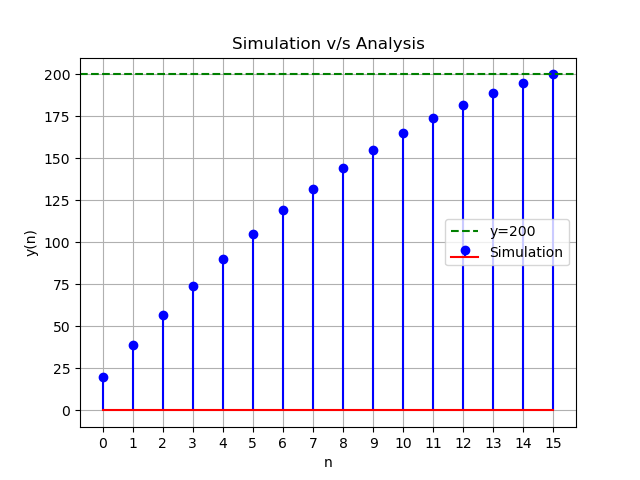
\includegraphics[width=1\linewidth]{/root/assign2/figs/figure_plot.png}
    \caption{plot of y\brak{n} v/s n}
    \label{fig:enter-label}
\end{figure}
\end{document}
